
% \begin{refsection}

% \newrefcontext[sorting=ynt]

\begin{center}
    \emph{What is a bird if not a dinosaur persevering?}
\end{center}

\medskip

\lettrine{B}{irds} are unique in moving mostly by powered flight on feathered wings.
Feathers, unlike animal hair and claws, are dead proteinaceous structures, which cannot be renewed continuously as they suffer wear and tear \parencite{rayner1988,jenni1989}.
As feathers mature, wing condition and consequently flight capacity gradually decreases \parencite{lindstrom1994,hedenstrom1999,hedenstrom2003}.
Moult --- the shedding of old, worn-out feathers, and their replacement with freshly grown ones --- is thus a key process in avian ecology \parencite{ginn1983,rayner1988}.
During wing moult, as one or more feathers are lost and new ones grow in their place, the flight surfaces of bird wings become smaller.
The reduction in flight surface area during moult can be measured using a robust-cross species index of the size of the (temporary) wing gap \citep{lind2001,kiat2016}.
Wider gaps lead to larger reductions in flight surface area, power output, and flight capacity and efficiency in captive birds \parencite{tucker1991,swaddle1996,swaddle1997,williams2003,lind2001,lind2001a,bowlin2009}.
In addition to these indirect costs, wing moult is among the most energetically demanding phases of a bird's annual cycle, as regrowing large flight feathers requires substantial resources \parencite{lindstrom1993,newton2009,kiat2017}.
Despite these mechanistic links between moult and movement, our understanding of moult's influence on birds' movement strategies and habitat selection is poor.

\graffito{
    Although I hadn't studied moult very much, I understood its effect on bird movement very well --- my master's fieldwork in Russia was timed to coincide with the full feather moult of white-fronted geese --- while flightless, they are easily chased down by humans.
}

The direct influence of wing moult on the movement and habitat selection of birds has primarily been examined in a few small-scale, disconnected studies \citep{bell1970,haukioja1971,green1975,francis1991,madsen1987,fox1998}.
Moving less, as some northerly species of finches and buntings do \citep{bell1970,haukioja1971,green1975,francis1991}, could save energy required to regrow feathers.
Avoiding predation risk during moult by sheltering in vegetation and rough terrain \citep{bell1970,haukioja1971,green1975,francis1991}, or near water-bodies as geese and ducks do \parencite{madsen1987,fox1998}, could also lead to reduced movement during moult.
Moult often coincides with migratory periods \citep{kiat2019}, making it difficult to separate the effects of migration-related energetic requirements \parencite{alerstam1990,wikelski2003,horvitz2014}, such as preferences for high-quality resources \parencite{madsen1987,fox1998}, from moult-related considerations on habitat selection.
Simultaneously, moult is influenced by bird physiology, with large-bodied species molting faster \citep{kiat2021,jenni2020}, and also by birds' evolved movement strategies, as wide-ranging and aerial foraging species (e.g., swifts and swallows) moult more slowly to maintain movement capacity \parencite{kiat2016}.

The direct effects of moult could be robustly studied with a cross-species comparison of unrelated, non-migratory species that are not constrained by the short time available for moult in northern temperate regions \parencite{ginn1983,jenni2020}.
Cross-species studies of movement and habitat selection in molting birds could benefit from dramatic advances in the high-throughput position tracking of small species \parencite{toledo2020,nathan2022}.
Birds, among other animals, can take the spatial perspective of visual predators, and avoid risky, exposed areas in favour of sheltered ones \parencite{hampton1994,emery2000,krams2001,davidson2016,krams2020}.
Shelter is often only proxied by correlated variables, such as vegetation growth \parencite{pettorelli2011}. 
Adopting a mechanistic, viewshed ecology approach \parencite{olsoy2015,aben2018,aben2021} in habitat selection analyses could directly account for birds' visibility to potential predators \parencite{olsoy2015,aben2018,aben2021}.

\graffito{I was heavily inspired to use the viewshed ecology approach after reading \textcite{aben2021}'s work on greenbuls (African forest bulbuls), and the methods I used here borrow heavily from that --- our advantage is combining that with fine-scale tracking.}

We explore the direct effects of wing moult on the movement of birds, focusing on four sympatric, non-migratory species: barn swallows (\textit{Hirundo rustica}), white-spectacled bulbuls (\textit{Pycnonotus xanthopygos}), house sparrows (\textit{Passer domesticus}), and clamorous reed-warblers (\textit{Acrocephalus stentoreus}).
Scoring the moult-related wing gap size of naturally molting birds \citep{lind2001,kiat2016}, we manipulated a subset of molting individuals by trimming a number of flight feathers.
We tracked birds during a 4-month period using the high-throughput ATLAS system, which brings unprecedented temporal and spatial resolution to small bird tracking \citep{toledo2014,weiser2016,toledo2020,nathan2022,beardsworth2022mee}.
We examined \textit{(i)} how the size of the moult-related wing gap affected bird movement, and \textit{(ii)} how the wing gap size influenced selection for more sheltered habitats.
Overall, we show how birds' movement decisions, influenced by their immediate physiological condition, scale up to affect their space use, and how individuals' adaptive behavioral strategies have feedbacks with their evolutionary ecology.

\section*{Examining the Movement of Moulting Birds}

We studied bird moult and movement in the Hula Valley of northern Israel (33.10°N, 35.60°E), which includes reconstructed wetlands and reedbeds as well as agricultural areas (crops, plantations and fishponds; see \textit{Supplementary Information}).

\subsection*{Bird Capture, Wing Moult Scoring and Experimental Manipulation}

We captured 86 individuals of four species in 2016: 16 barn swallows, 19 white-spectacled bulbuls, 35 house sparrows, and 16 clamorous reed-warblers, for which we also measured the wing gap index.
All individuals were trapped after breeding was completed and before the molting season commenced, between June and October 2016.

We described the state of each primary feather on a scale of 0 to 5 using the primary score (PS) method \citep{ginn1983}.
Both PS = 0 and PS = 5 indicate a fully mature feather, and hence no gap in the wing.
A PS value between 1 and 4 indicates feathers in increasing stages of growth, with PS = 1 representing a large gap left by a recently molted feather.
This method allows a cross-species estimate of the size of the moult-related gap in the wing, and is also strongly and negatively correlated with moult rate and duration \citep{rohwer2009}.
We scored the wing gap size due to any single feather molting as the inverse value of PS for each of the wing's nine primary feathers (P1 -- P9; counted outward) such that when PS = 1, wing gap size = 4, and when PS = 2, wing gap size = 3, etc.
However, for PS = 0, wing gap size is also 0 because there is no gap in both the PS = 0 and PS = 5 stages, as either an old, mature feather, or a new, freshly grown feather is present.
To compare moult-related wing gap sizes across individual birds, we summed the wing gap size scores across all nine primary flight feathers, for each individual, into a single wing gap index \citep{kiat2016}.
This index is independent of the size of individual birds and their morphology, controls for the stage of wing feather moult, and allows for reliable cross-species comparisons \citep{bensch1993,kiat2016}.

\graffito{
    All the fieldwork for this study --- setting up the ATLAS system in the Hula Valley, capturing birds, measuring the extent of wing moult, and fitting them with ATLAS tags --- was performed by my co-authors in Israel. Special thanks also go to Yotam Orchan, who was responsible for managing the ATLAS system in the field.
}

We experimentally manipulated 29 individuals across species {(bulbuls = 6, sparrows = 14, reed-warblers = 2, swallows = 7)}, and removed one to three primaries; the exact number was determined randomly for each bird.
We varied this number to produce variation in the possible effect of wing gap size, and the manipulation was symmetrical, i.e., the same feather was removed in both wings.
Primaries were removed by cutting the feather near its base, in addition to the primaries missing as part of natural moult; this procedure simulates an enlargement of the moult-related wing gap.
Cutting the feather rather than tearing it out from the base, which is still innervated \parencite{jenni2020}, avoided excess trauma which could impact birds' behaviour, and allowed us to examine the effect of only the wing gap size on movement and habitat selection.
For these experimentally manipulated birds, we calculated the wing gap size after the procedure described here.
Bird capture and handling, the experimental manipulation procedure, and tagging for position tracking (see below) were conducted under a permit from the Israel Nature and Parks Authority (NPA permit 2016/41402) and from the ethics committee of the Hebrew University of Jerusalem, Israel (NS-16-14801-2).

\subsection*{Forecasting Daily Changes in the Wing Gap Size Index}

The size of the moult-related wing gap decreases slowly and constantly as feathers regrow, yet as a mature feather is shed, the wing gap size may also increase in gradual jumps.
Over our tracking period of about 7 days per individual (see below), this is expected to represent small changes in the wing surface area, which could further influence movement decisions.
These changes in wing condition should be accounted for when relating movement characteristics to wing gap size.
To do this, we calculated for each species the mean daily progress in the moult score, based on a sample of individuals documented twice during the moult process (bulbul = 0.45 $\pm$ 0.15, n = 17; sparrow = 0.40 $\pm$ 0.25, n = 10; reed-warbler = 0.69 $\pm$ 0.34, n = 24; swallow = 0.34 $\pm$ 0.18, n = 22). 
Then, we estimated for each bird included in the study the expected daily change based on the measurement we made at the time of tagging (see \textit{Supplementary Information}).

\subsection*{Tracking Bird Movement Using ATLAS}

We tracked the movement of individual birds using ATLAS (Advanced Tracking and Localization of Animals in real-life Systems), a state-of-the-art high-throughput radio-telemetry system capable of tracking dozens of individuals at intervals as low as 4 seconds \citep{weiser2016,toledo2014,toledo2020,nathan2022}.
We glued ATLAS tags (0.9 -- 1.6 g, depending on species) to birds' dorsal feathers after capture, and then released them (tag weights as percent of body mass: bulbuls = 3.85\% $\pm$ 0.21\%; sparrows = 4.21 $\pm$ 0.13; reed-warblers = 4.75\% $\pm$ 0.19\%; swallows = 4.9\% $\pm$ 0.13\%).
Tags automatically drop off as these feathers are molted.
Each individual was tracked for an average of 8.23 $\pm$ 3.24 days (bulbul = 9.8 $\pm$ 10.1 days; sparrow = 12.0 $\pm$ 13.4 days; reed-warbler = 5.9 $\pm$ 2.1 days; swallow = 5.1 $\pm$ 14.8 days).
We collected 4.3 million position estimates overall, with 7,276 positions per individual per day, for an effective tracking interval of 5.05 $\pm$ 1.85 positions per minute on average (bulbuls = 6.14 $\pm$ 3.93; sparrows = 5.98 $\pm$ 5.57; reed warblers = 5.80 $\pm$ 3.16; swallows = 2.28 $\pm$ 1.42).
Since we were interested in exploring movement patterns, and these species are diurnally active, we removed all nighttime positions, leading to an approximate halving of the total dataset.

\graffito{
    This study uses data from 2016, when the ATLAS system was still in its infancy. The system is constantly being improved, with upgrades to the hardware to make tags lighter and longer lasting, as well as software updates that make localisations more accurate.
}

\subsection*{Processing Tracking Data}

ATLAS conservatively filters out location estimates that are clearly wrong (e.g., too far from the study area), letting users inspect most location estimates, which come with several measures of quality, 
% (estimated covariance matrix, quality of fit to constraints, and the norm of the gradient of the objective function), 
and decide whether they want to retain the estimates or not. 
For this study, we aggressively filtered out location estimates, removing estimates for which we had indications that ATLAS failed to find a high-quality estimate \citep{gupte2022d} (see \emph{log\_preprocessing.log} in the analysis code).
We began data cleaning by removing locations near a so-called attractor position (at (257000.0,780000.0), Israeli grid; see file \textit{log\_preprocessing.log}); these are locations for which the positioning system had defaulted to a (wrong) estimate.
We identified and removed other attractor positions by removing positions sharing the exact same common coordinate pair. 
Since coordinates are resolved down to double-precision, it is very unlikely for two location estimates to have the same coordinate pair, and this rather indicates an error in location estimation.
Each individual's track was pre-processed separately.

We first \textit{(i)} filtered the data for large-scale errors by removing positions with a system-generated positioning-error estimate (SD) $>$ 20m, and then \textit{(ii)} split each individual's tracking data by calendar date, removing days with $<$ 500 positions. 
Finally, we \textit{(iii)} filtered the data for unrealistic movements, removing positions with both speeds $>$ 20 m/s \emph{and} a turning angle >10\textdegree.
We deliberately used larger thresholds than these species' maximum speeds to avoid removing valid, high-speed movements \citep{gupte2022d}.
Finally, we \textit{(iv)} accounted for small-scale errors --- noise around the true positions --- by applying a median smooth with a moving window $K$ = 7.
After excluding night time data and all other data filtering and smoothing, we analyzed 1.1 million locations from 86 individuals, keeping high per-minute sampling rate for all species (bulbuls = 4.85 $\pm$ 3.3, sparrows = 2.73 $\pm$ 3.0, reed-warblers = 2.09 $\pm$ 1.44, swallows = 2.07 $\pm$ 1.14).
Compared with current technologies for tracking small birds ($<$ 50g) --- primarily radio triangulation and geolocators, which have low temporal (a few fixes per hour or day) and spatial resolution (error margins up to 200 km) \citep{bridge2013} --- ATLAS data represent an unprecedented sampling rate, with GPS-level accuracy \citep{beardsworth2022mee}.

\graffito{
    Of course, one downside here is the relatively small spatial extent of the area that ATLAS can cover. Yet for mostly sedentary birds such as bulbuls and reed warblers, even a localised system is able to capture the entire home range.
}

\subsection*{Quantifying Large-scale Movements}

We investigated the large-scale space-use of bulbuls, sparrows, and reed-warblers by summarising their processed movement paths into daily sequences of `residence patches' using the \textit{atlastools} package developed specifically with high-throughput ATLAS tracking data in mind \citep{gupte2022d}.
The residence patch algorithm uses simple distance and duration thresholds, chosen based on the movement ecology of the tracked species, to efficiently and rapidly cluster-segment individuals' non-travelling positions \citep{gupte2022d}.
We applied this algorithm to the date-specific tracks of each individual, considering consecutive positions less than 25m and 30 minutes apart to be part of the same cluster.
We joined clusters (with at least 9 positions) less than 100m and 30 minutes apart together for bulbuls and sparrows, and less than 25m and 30 minutes apart for reed warblers, which typically fly only short distances \parencite{kiat2016}.
Doing so, we obtained 4,373 residence patches overall and extracted environmental covariates (NDVI and visibility index; see below) for the positions clustered into each patch.
%%
We handled swallows differently, as these are highly aerial birds whose movement is not easily clustered into residence patches.
Instead, and because the relatively higher-flying swallows are more accurately tracked by ATLAS, we simply calculated the total distances moved along daily tracks from the cleaned, processed data.

\graffito{See Chapter~\ref{ch:preprocessing} for more details on pre-processing, as well as on the residence patch algorithm.}

\subsection*{Visibility Analysis to Quantify Sheltered Habitats}

Many animals can gauge the risk posed by predators by estimating a predator's field of view (`spatial perspective taking') \parencite{emery2000,bruce2003,davidson2016}, and select for sheltered locations outside of a predator's view \citep{hampton1994,krams2001,watve2002}.
To assess the field of view of a hypothetical predator, and thus the estimated riskiness of the landscape, we took a viewshed ecology approach to determine how visible an area was from surrounding locations \citep{aben2018,aben2021}.

We first obtained a 50cm canopy height model (CHM) \citep{aben2021} of the majority of our study area (courtesy of the Survey of Israel).
For each cell of the CHM, we calculated a \textit{visibility index}, which is the proportion of surrounding cells from which the focal cell is visible, given that lines of sight can be blocked by intervening structures (also called cumulative viewshed analysis, or a `fearscape') \parencite{olsoy2015}.
Open areas, such as agricultural fields or water bodies, are likely to be visible from all directions and have a visibility score $\approx$ 1.0.
In contrast, locations inside woodland or reedbeds are likely to be hidden from view, with a lower visibility index (see \textit{Supplementary Information}).

\graffito{
    We initially thought that we would not be able to obtain the CHM from the Survey of Israel, as the Hula Valley is in a border region. However, we did manage to get almost the entire study area in excellent resolution, for which we thank the Survey.
}

Importantly, the visibility index depends upon the hypothetical observer's height above surface level; observers higher up may be able to see locations that are obstructed from a terrestrial viewpoint.
We parameterised our visibility index calculations based on the hunting flight altitude of a raptor that commonly preys on small birds, the Eurasian sparrowhawk (\textit{Accipiter nisus}).
Sparrowhawks and other bird-preying raptors hunt by surprising their prey via low-level flight, as hovering or high-flying raptors are conspicuous and can be easily detected \parencite{krams2001,krams2020}.
In line with experimental and observational work, we assumed an observer height of 1.5m above surfaces (tree canopy, fields, or other) \citep{seress2011,krams2020}, and an observer visual range of 50m.
We used the `Visibility Analysis' plugin v1.2 for QGIS v3.20 to calculate visibility scores over the study area \citep{cuckovic2016}.

\subsection*{Drawing Alternative Residence Patches to Examine Habitat Selection}

In our landscape, it is mostly wooded areas that offer shelter from observation by aerial predators (see \textit{Supplementary Information}).
We examined the relative importance of the provisioning effects of vegetation (proxied by NDVI) \parencite{pettorelli2011}, and its sheltering effects (section F above), on birds' movement decisions at the patch scale.
To do this, we combined our residence patch approach for bulbuls, sparrows, and reed warblers with a step-selection approach \citep{thurfjell2014,avgar2016} using the \textit{amt} package \citep{signer2019}.
While barn swallows could potentially make use of sheltering vegetation by flying very low \parencite{warrick2016}, we could not detect their altitude above the ground --- a key component of shelter --- and so did not include them in this analysis.

We first converted each individual's daily sequence of residence patches into steps, with each patch $i$ as the starting point, and the following patch $i+1$ as the end of the step.
Then, for each such real step, we drew 9 alternative steps that the individual could have taken from patch $i$, and considered the end coordinates of these alternative steps to represent the median coordinates of a potential residence patch.
The distances of these movements were drawn from a gamma distribution fitted to each individual's movements between patches, and turning angles were drawn from a von Mises distributions fitted to the observed turning angles \citep{signer2019}.
For each alternative patch with median coordinates ($X_\text{alt}, Y_\text{alt}$), we drew 15 coordinate pairs from a normal distribution centred on ($X_\text{alt}, Y_\text{alt}$), with a standard deviation of 20 m.

\graffito{
    Level 1C data is from the so-called Top of Atmosphere (ToA), in contrast with the better quality Level 2A data, which correct for sensor distortions created by some dozens of kilometers of the atmosphere between the land surface and the satellite. 2A data are only available from 2017 onwards, which means that studies like ours that need spectal indices from before that must use 1C data.
}

To control for the resource-provisioning effect of vegetation, we also obtained the normalised difference vegetation index (NDVI) as a metric of vegetation growth \citep{pettorelli2011} across our study area, using Copernicus Sentinel-2 MultiSpectral Instrument, Level-1C data (10m resolution; June -- October 2016).
We sampled the NDVI and visibility index at real and potential patch coordinates, and calculated averages per patch.
With between-patch movements as steps, we performed species- and moult-status specific step-selection analysis (SSA) to determine how these predictors affected habitat selection \parencite[][see \textit{Supplementary Information}]{avgar2016}.
The time intervals between patches were not fixed, but step lengths were not dependent on step duration, and so we implemented a simple SSA.

\section*{Effect of Wing Moult on Bird Movement and Habitat Selection}

\subsection*{Moult-related wing gap size}

\begin{figure}[!t]
\centering
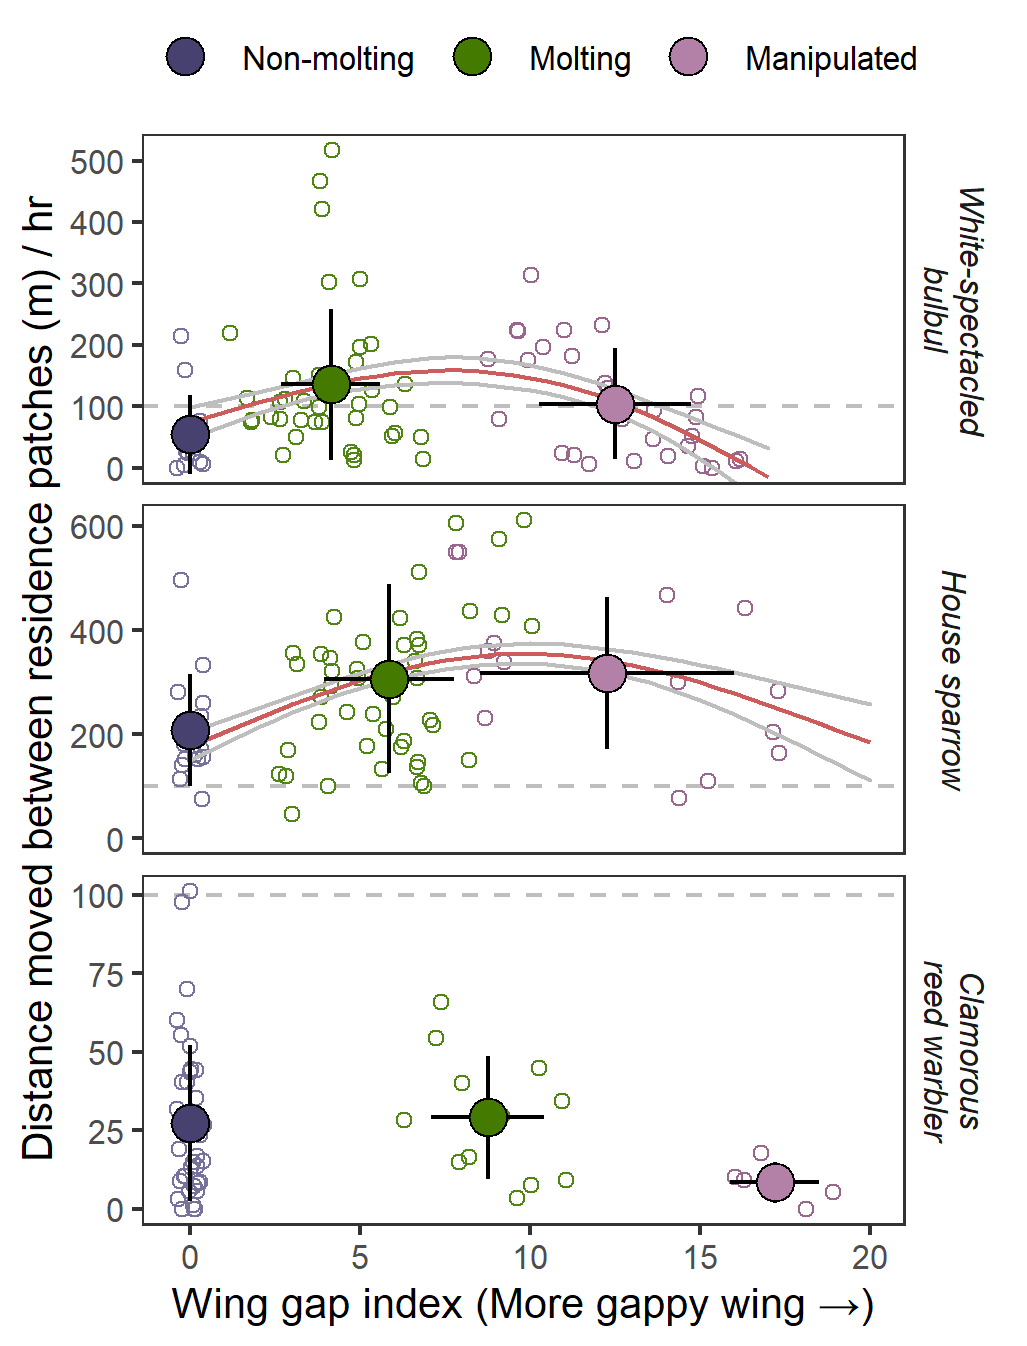
\includegraphics[0.9\textwidth]{figures/holeybirds/fig_01.png}
\caption{
    \textbf{Naturally molting bulbuls and sparrows, but not reed-warblers, move farther between residence patches during natural moult than following experimental feather manipulation.}
    White-spectacled bulbuls (\textit{Pycnonotus xanthopygos}) and house sparrows (\textit{Passer domesticus}) moved 251\% and 150\% as far between areas of prolonged use (`residence patches') when molting, compared to non-molting individuals (see text for statistics).
    %generalised additive model estimates: bulbuls, $F$ = 4.734, p = 0.01; sparrows, $F$ = 11.58, p < 0.001).
    However, when bulbuls' and sparrows' wings were heavily compromised by experimental manipulation (wing gap index $\geq$ 12), both species made shorter movements between residence patches.
    In contrast, clamorous reed-warblers (\textit{Acrocephalus stentoreus}) did not show a significant difference in large-scale movements with increasing wing gap index, possibly because they are already restricted to small patches of reedbeds.
}\label{holey_fig_01}
\end{figure}

Of the four species we studied, bulbuls and sparrows are relatively wide-ranging birds, reed-warblers are strongly range restricted to patchy reedbeds, and swallows are very wide-ranging, largely aerial foragers.
Bulbuls and sparrows moult more slowly than reed-warblers, but more rapidly than swallows.
Thus reed-warblers have the largest moult-related wing gaps, swallows the smallest, while bulbuls and sparrows are intermediate between them {(wing gap index, mean $\pm$ SD: swallows = 4.3 $\pm$ 0.95, bulbuls = 4.95 $\pm$ 1.37, sparrows = 5.9 $\pm$ 2.1, reed warblers = 9.5 $\pm$ 1.38)}.
All non-molting birds had a wing gap index score of zero.

\subsection*{Moult-related Wing Gap Size and Large-scale Movements}

For bulbuls, sparrows, and reed-warblers, we quantified large-scale movements as both the displacements between areas of prolonged residence, called `residence patches' \parencite{gupte2022d}, as well as the frequency of these displacements.
Since swallows constantly fly while foraging, we chose to quantify their large-scale movement by simply calculating the total distance moved, adjusting for the daily duration of daytime tracking.
We related total large-scale movements (controlling for daily, daytime tracking duration) with wing gap size using generalised additive models (GAM).
We fit one GAM for bulbuls, sparrows, and reed-warblers (species included as both fixed and random effect), and a separate GAM for swallows (see \textit{Methods}; see \textit{Supplementary Information} for model specification).

\begin{figure}[!t]
    \centering
    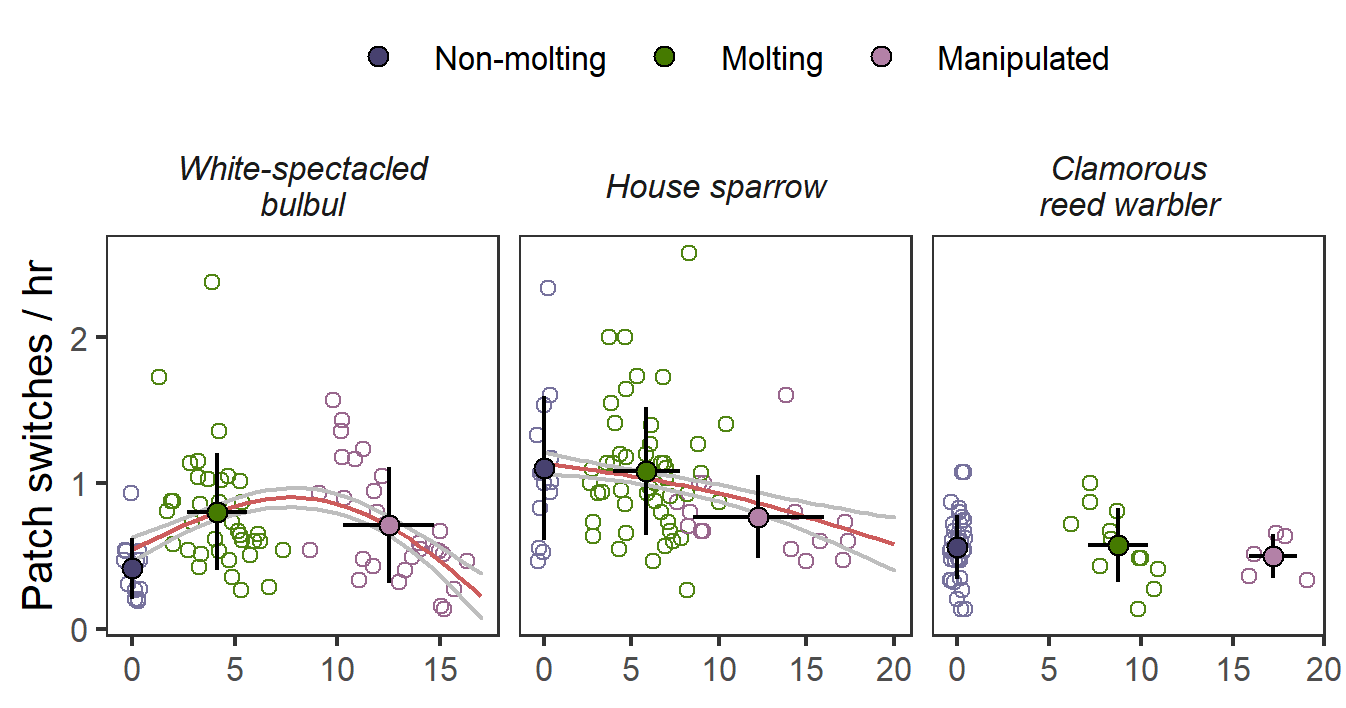
\includegraphics[0.9\textwidth]{figures/holeybirds/fig_02.png}
    % width=8.7cm,height=8.7cm
    \caption{
        \textbf{Patch-switching behaviour is affected by wing gap size in bulbuls and sparrows, but not in reed-warblers.}
        Bulbuls switched between areas of prolonged use (`residence patches') more frequently when molting naturally than when not molting; however, bulbuls whose feathers had been artificially cut (`manipulated') switched less frequently between patches.
        %(generalised additive model [GAM] estimates: $F$ = 7.45, p $<$ 0.001).
        Molting sparrows switched residence patches less frequently with increasing wing gap index; naturally molting birds switched less than non-molting ones, and manipulated birds least of all. %(GAM estimates: $F$ = 3.52, p = 0.024).
        Reed-warblers did not show a significant difference in patch switching with increasing wing gap index, possibly because they are already restricted to small patches of reedbeds.
    }\label{holey_fig_02}
\end{figure}

\graffito{Throughout this paper I've chosen to use the Batlow colour scheme from the `scico' package for perceptually uniform colour palettes in R. The key was to choose colours without semantic meaning, such as blue or red; a similar consideration led to the colours used in Chapter~\ref{ch:preprocessing}.}

\subsection*{Distance Between Residence Patches}

We found that bulbuls and sparrows, but not reed-warblers, adjusted their daytime large-scale movements between residence patches to their wing gap size (Fig.~\ref{holey_fig_01}; GAM t-value = 2.13, p = 0.034; \textit{Supplementary Information} Table~\ref{table:coef_distance}).
Compared with non-molting individuals (wing gap = 0), naturally molting bulbuls with moderately large moult-related gaps (3 $<$ wing gap $\leq$ 10) actually moved 2.5 times as far per hour between residence patches (GAM estimate $F$ = 4.734, p = 0.01; distance between patches: non-molting = 54.11 m, molting = 135.89 m).
Similarly, naturally molting sparrows moved {1.5 times} as far per hour between residence patches (GAM estimate $F$ = 11.58, p = 0.00002; distance between patches: non-molting = 208 m, molting = 307 m).
This is consistent with the idea that wing moult is an energetically demanding period that requires actively seeking out high-quality food sources \citep{madsen1987,fox1998}.

Reed-warblers and swallows, which represent very rapid and very slow moult rates, respectively, showed no statistically significant change in large-scale movement with increasing size of the moult-related wing gap (Fig.~\ref{holey_fig_01}: reed-warblers).
Rapidly-molting reed-warblers moved similar distances between residence patches when molting or non-molting (GAM estimate $F$ = 0.055, p = 0.815; Fig.~\ref{holey_fig_01}).
This is presumably because reed-warblers 
% are already very strongly constrained to a few clustered reedbed habitats, and thus 
do not move between distant patches even when not molting (mean distance between residence patches: non-molting = 27.20 m, molting = 29.09 m, manipulated = 8.49 m) \citep{kiat2016}.
Slow-molting swallows also moved similar (large) distances per hour when they were either non-molting, molting, or artificially manipulated (GAM estimate $F$ = 0.129, p = 0.723).
Swallows' slow moult rate likely represents an adaptation to their aerial foraging habit, allowing them to maintain flight performance across moult stages (non-molting = 3.48 $\pm$ 1.36 km, molting = 3.36 $\pm$ 1.17 km, manipulated = 3.64 $\pm$ 1.96 km).

\subsection*{Effect of Artificial Manipulation}

Our experimental manipulation involved removal of one to three primaries, in addition to the primaries missing as part of natural moult (see \emph{Methods}).
Wing gap index scores after artificial manipulation showed differences among species corresponding to their natural moult rate, manipulated reed warblers had larger wing gaps than manipulated swallows, bulbuls, or sparrows {(swallows = 10.11 $\pm$ 2.5, bulbuls = 13.5 $\pm$ 2.35, sparrows = 12.56 $\pm$ 3.5, reed-warblers = 17.8 $\pm$ 1.1).}
Bulbuls and sparrows whose flight feathers had been removed by manipulation (12 $<$ wing gap $<$ 20) moved shorter distances than naturally molting birds {(bulbuls: 68\% less, 43 m; sparrows: 16.7\% less, 256 m)}.
% Bulbuls especially barely moved at all between residence patches when their wings were heavily compromised by artificial manipulation (wing gap $>$ 15; mean distance between residence patches / hr = 39.3 $\pm$ 42.2 m; Fig.~\ref{holey_fig_01}).
These observations are in line with the direct effects of severely reduced flight capacity and allocating energy reserves to feather regrowth rather than movement, and an indirect effect of risk-avoidance during a vulnerable period.

\subsection*{Frequency of Patch Switching}

We found that in addition to affecting the distance moved between residence patches, the wing gap resulting from natural moult or manipulation also affected the frequency of patch switching in bulbuls and sparrows, but not in reed-warblers (Fig.~\ref{holey_fig_02}).
Naturally molting bulbuls moved more often between residence patches than non-molting and artifically manipulated birds (GAM estimate $F$ = 7.45, p $<$ 0.001; see also \textit{Supplementary Information} Table~\ref{table:coef_switches}).
However, naturally molting sparrows switched between residence patches as often as non-molting birds, but artificially manipulated sparrows switched patches less frequently than molting birds (GAM estimate $F$ = 3.515, p = 0.024; Fig.~\ref{holey_fig_02}).
Reed-warblers did not show a change in patch-switching frequency in relation to wing gap size (GAM estimate $F$ = 1.04, p = 0.31).

\begin{figure}[!t]
    \centering
    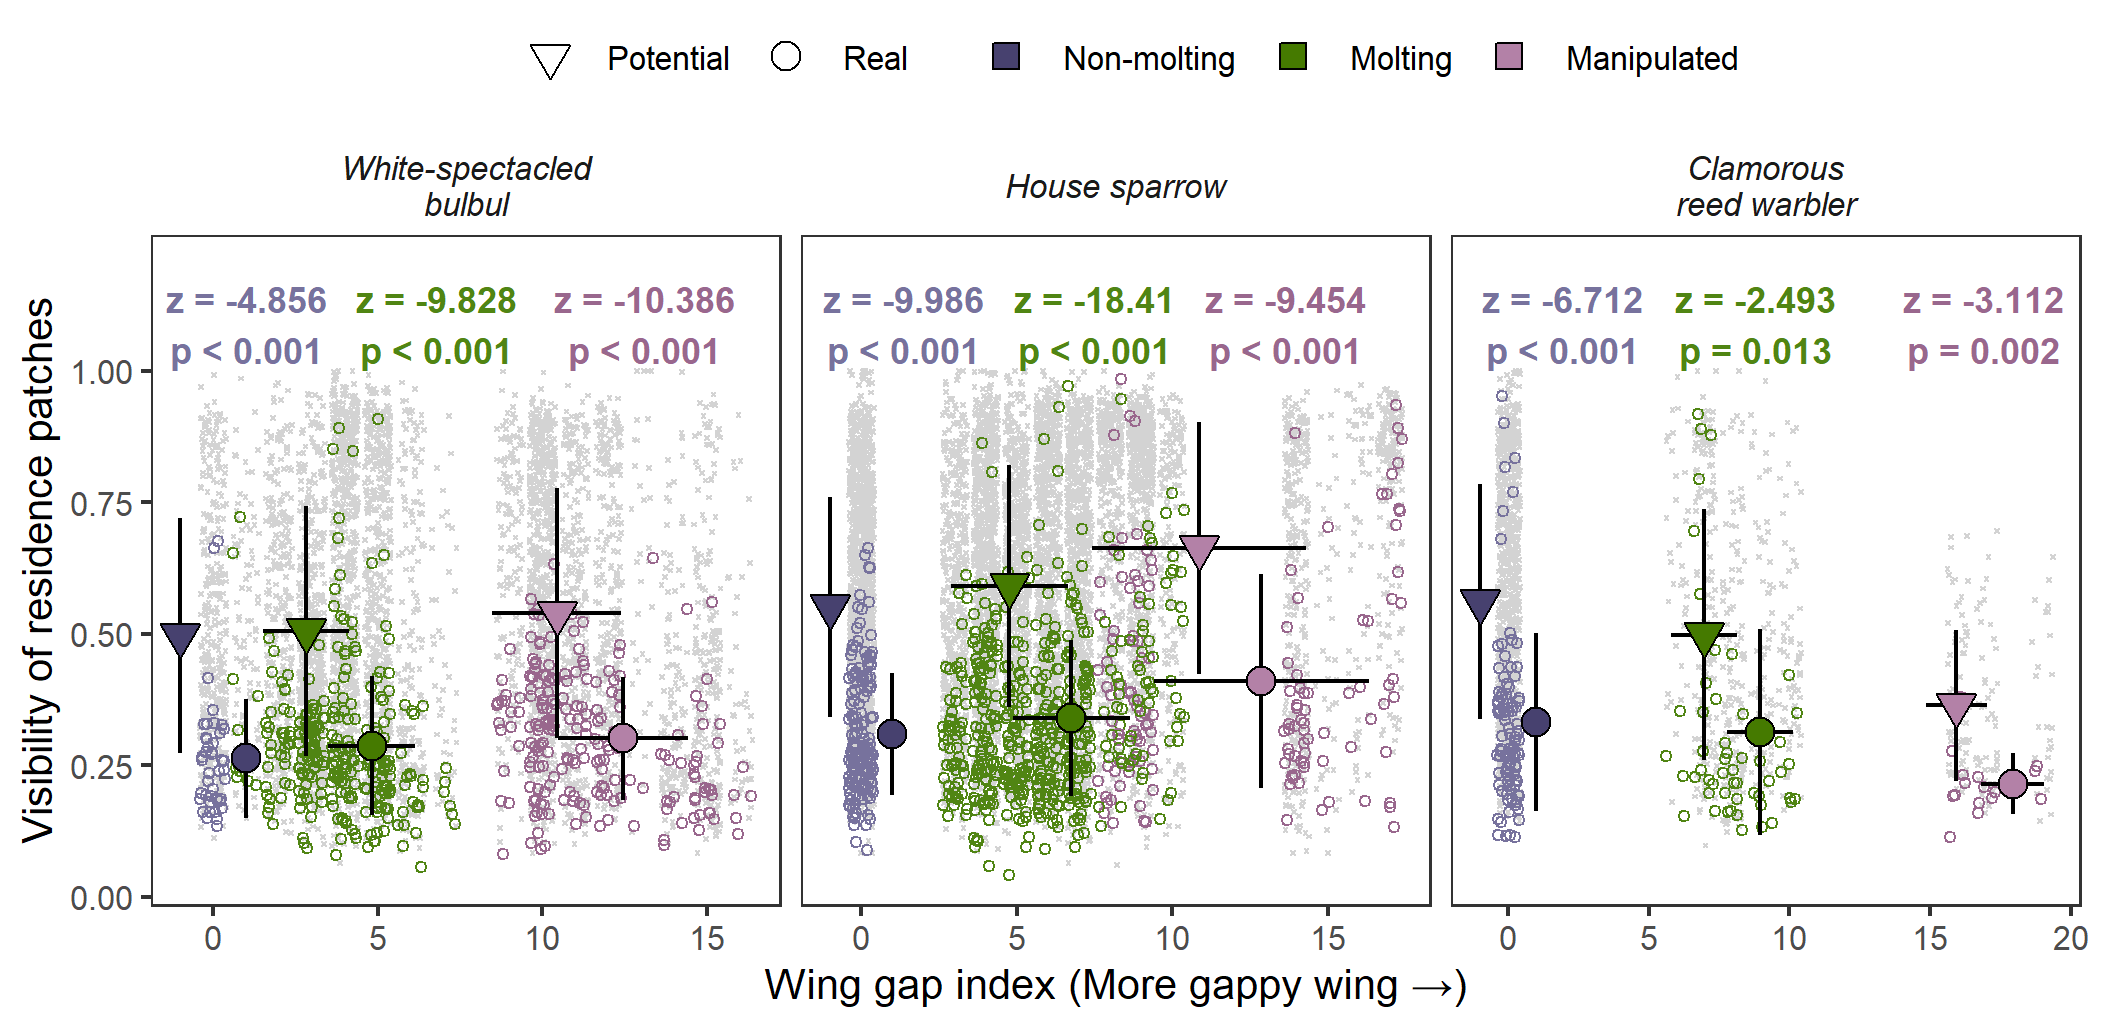
\includegraphics[0.9\textwidth]{figures/holeybirds/fig_03.png}
    % width=8.7cm,height=8.7cm
    \caption{
        \textbf{Naturally molting bulbuls and reed-warblers, but not sparrows, use residence patches for shorter durations than non-molting and artificially manipulated birds.}
        Bulbuls and reed-warblers use contiguous areas for shorter durations when molting, than either when not molting or when some of their flight feathers have been removed by artificial manipulation. 
        %(GAM estimates: bulbuls, $F$ = 18.87, p $<$ 0.001; warblers, $F$ = 12.85, p $<$ 0.001).
        However, sparrows did not show an effect of wing condition on their use of residence patches. %(GAM estimate $F$ = 0.02, p = 0.88).
        The visibility of a patch to low-flying predators reduced the duration for which it was used, %(GAM parametric estimate = -0.70, p = 0.004), 
        but patch vegetation productivity (NDVI) had no effect. 
        %(GAM parametric estimate = 0.05, p = 0.86).
    }\label{holey_fig_03}
\end{figure}

\subsection*{Moult-related Wing Gap size and Patch Occupancy}

We examined whether the time that bird spent in residence patches was affected by their wing gap size, with the expectation --- following the results for movements between patches --- that molting birds would spend less time in patches than non-molting and manipulated birds (see \textit{Supplementary Information} for model specification).
This was indeed the case for both bulbuls and reed-warblers, for which the mean patch duration for molting birds was only about half of that for non-molting and manipulated birds (Fig.~\ref{holey_fig_03}; GAM estimates: bulbuls, $F$ = 18.86, p $<$ 0.001; reed warblers, $F$ = 12.854, p $<$ 0.001).
However, we found that sparrows had similar patch durations across different wing gap sizes (GAM estimate $F$ = 0.023, p = 0.878; \textit{Supplementary Information} Table~\ref{table:coef_duration}).

We expected two environmental attributes --- vegetation productivity (NDVI), and visibility to predators --- to also affect patch durations.
To quantify patch visibility, we calculated the visibility index across our study area \parencite{olsoy2015,aben2018,aben2021}.
The visibility index represents whether a location can be observed from surrounding areas, for example by a commonly occurring predator, the Eurasian Sparrowhawk (\textit{Accipiter nisus}; see \textit{Methods}).
Areas with taller vegetation such as orchards, and built-up areas such as settlements have lower visibility indices and are more sheltered (see \textit{Supplementary Information}), as predators' lines of sight are obstructed by intervening objects \parencite{olsoy2015}.
We found that NDVI did not appear to influence patch duration (GAM parametric estimate = 0.056, p = 0.86).
However, patch durations increased with reduced patch visibility (GAM parametric estimate = -0.70, p = 0.004).

\subsection*{Birds Occupy Sheltered Areas across Moult Rates}

Finding that patch visibility influenced patch durations, we examined whether birds' moult-related wing gaps directly influenced their use of sheltered areas (except swallows, which are aerial foragers).
First, fitting a GAM with species-specific smooths for bulbuls, sparrows, and reed-warblers (see \textit{Methods}), we found that only reed-warblers had slightly more sheltered patches with larger wing gaps (GAM estimate $F$ = 9.30, p = 0.002; Fig.~\ref{holey_fig_04}; visibility: non-molting = 0.33 $\pm$ 0.17, molting = 0.31 $\pm$ 0.19, manipulated = 0.21 $\pm$ 0.06), potentially because their rapid moult rate severely reduces flight capacity and makes increased shelter necessary.
% only a moderate overall relationship between the visibility index of residence patches and the size of the moult-related wing gap (GAM t-value = 100.5, p $<$ 0.001; $R^2$ = 0.312).
This suggests that bulbuls and sparrows, with intermediate moult rates, occupy sheltered areas of similar (low) visibility regardless of the size of their wing gap (visibility: bulbuls =  0.39 $\pm$ 0.18; sparrows = 0.47 $\pm$ 0.19; see \textit{Supplementary Information} Table~\ref{table:coef_vis}).

We went one step further, and used a step-selection approach to sample patches to which individuals could have moved, and estimated birds' relative preference for visibility and NDVI when making movement decisions (see \textit{Methods}) \citep{avgar2016,aben2021}.
Fitting separate step-selection functions for each species and each broad moult group (non-molting, molting, and manipulated), we found that across moult group, all three species preferred low-visibility sheltered sites over higher visibility ones (Fig.~\ref{holey_fig_04}; \textit{Supplementary Information} Table S5).
Furthermore, NDVI did not signficantly affect birds' movement decisions at the patch scale (see \textit{Supplementary Information} Table {S1}).
This is consistent with the idea that birds of our study species mostly avoid open agricultural fields, where they might be exposed to potential predators, even though fields are highly productive.

\afterpage{
    \begin{sidewaysfigure}[p]
        \centering
        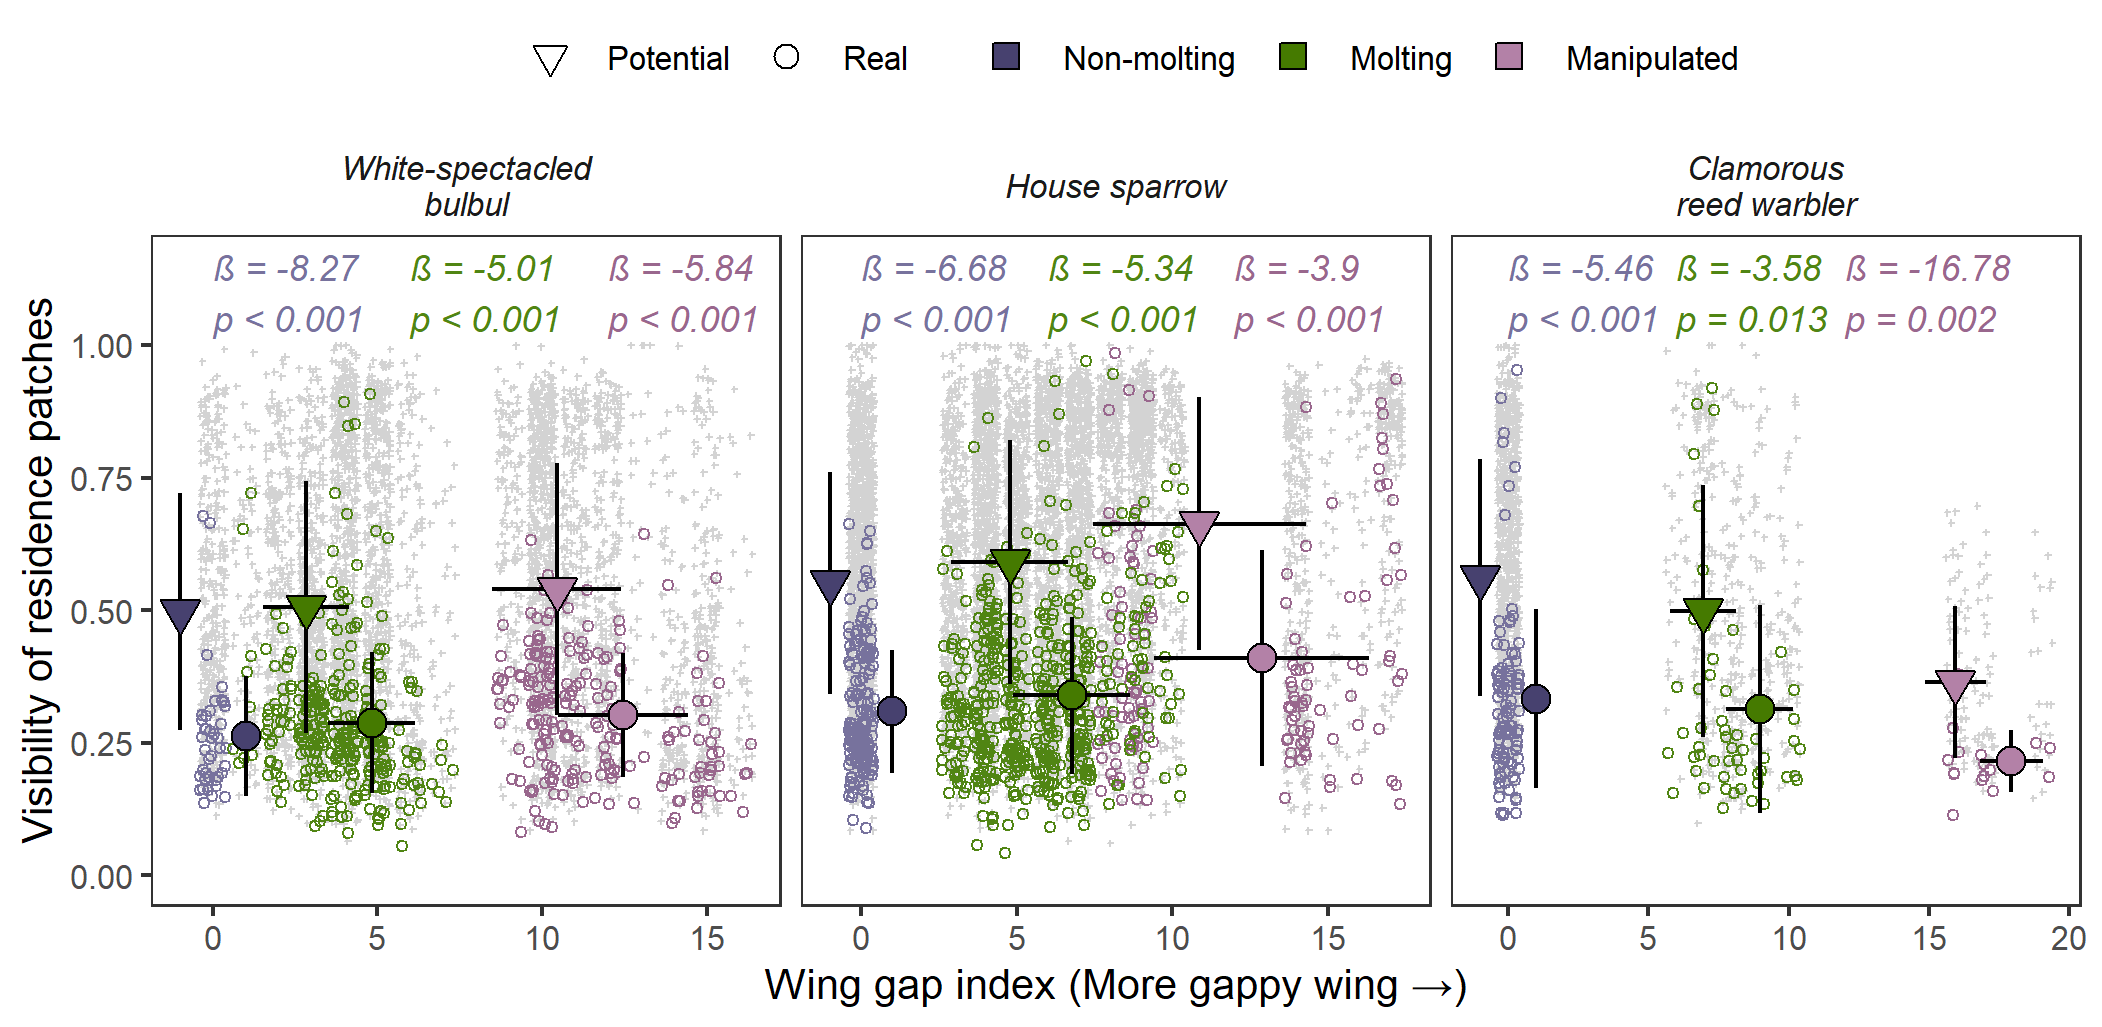
\includegraphics[0.7\textwidth]{figures/holeybirds/fig_04.png}
        % width=8.7cm,height=8.7cm
        \caption{
            \textbf{Bulbuls, sparrows, and reed-warblers prefer sheltered habitats across wing condition.}
            Across the three species, a GAM indicated that moult-related wing gap index was a poor predictor of the visibility of areas actually occupied by individuals (`real' residence patches; small colored circles). 
            A step-selection analysis at patch level, comparing real residence patches to sampled potential residence patches (grey crosses), showed strong selection for patches with low visibility index scores for all wing conditions, indicated by negative estimated selection coefficients ($\beta$ = natural logarithm of relative selection strength). 
            All $\beta$ values were statistically significant (see \textit{Supplementary Information}).
            Filled circles and triangles, and error bars around them, show the mean visibility index of real and potential patches for each moult treatment (indicated by color).
        }\label{holey_fig_04}
    \end{sidewaysfigure}
}

\section*{Interpreting the Effect of Wing Moult on Bird Movement}

Our study is among the first to quantify how the compromised wing surface associated with moult directly affects movement and habitat selection in wild birds.
Our high-throughput tracking system enabled tracking small birds at temporal (several times per minute) and spatial resolutions (a few metres) far surpassing current technologies for tracking such small birds ($<$ 50g) --- mainly through radio triangulation and geolocators, that have low temporal (a few fixes per hour or day, respectively) and spatial resolution (error margins up to 200 km) \citep{bridge2013}.
Focusing on resident birds outside their breeding season, rather than migratory or breeding ones, enables at least some control on confounding factors associated with seasonal physiological changes, and the confounding effect of migration- or breeding-related energy and time requirements \parencite{alerstam1990,wikelski2003,horvitz2014}.
Our study also extends the geographic range of the field to an understudied region, and to two less-studied species.

Both rapidly molting clamorous reed-warblers, and slow-molting barn swallows, did not adjust their large-scale movements to their wing condition.
Reed-warblers move very short distances ($<$ 25m) in low-visibility areas, and can afford rapid, resource-intensive feather growth \citep{lindstrom1993,newton2009,kiat2017}, as this does not compromise their ability to move scansorially through their dense reedbed habitat, which also offers shelter from visual predators.
At the other extreme, barn swallows that forage exclusively while flying have evolved a very slow moult rate \parencite{kiat2016}, which likely forestalls significant direct aerodynamic effects of feather loss on flight capacity.
Our work shows how birds' evolved moult strategies --- which are themselves influenced by movement strategies \parencite{kiat2016} --- are interlinked with the direct, short-term effects of moult on movement.

We also found that birds with intermediate moult rates --- white-spectacled bulbuls and house sparrows --- adapt their movement strategies to their wing morphology.
Surprisingly, these species moved more when naturally molting than non-molting.
Birds can compensate for lower wing power output by growing their pectoral muscles, and this may allow them to maintain flight capacity during the moult, enabling increased movement to find resources for feather growth \parencite{chai1997,swaddle1997}.
Unsurprisingly, increased movements between putative foraging patches, and an increased frequency of such movements, together translate into a shorter occupancy duration in each patch.
While this movement strategy conforms with optimal foraging theory --- rapid abandonment of patches to maximise prey intake \parencite{charnov1976} --- it does not appear that vegetation productivity influences patch use.

When increased movement for high quality resources \parencite{charnov1976} cannot compensate for the costs of inefficient flight and feather growth, moving less overall to conserve energy may be the optimal strategy until new flight feathers develop.
This latter strategy should be expected when the wing gap size is increased beyond the extent of natural moult, as found in our study.
The shorter between-patch movements of artificially manipulated sparrows and bulbuls with especially large wing gaps (wing gap index $>$ 12), compared with natural moult, thus fit within this hypothesis.
Importantly, our relatively non-invasive method only increases the wing's feather gap size while avoiding wing injury, suggesting that the reduction in flight is actually due to considerations of flight efficiency, rather than trauma.

We have for the first time applied the idea of the cumulative viewshed to directly assess the availability of shelter from visual predators, along birds' real and potential movement paths \parencite{olsoy2015}.
Birds, like other animals, are capable of taking the spatial perspective of other individuals \parencite{emery2000,krams2001,watve2002,davidson2016}, i.e., whether a location would be visible to another observer, such as a predator \citep{watve2002,olsoy2015}.
Previous work has focused on demonstrating spatial perspective taking --- and resulting habitat selection --- at small spatial scales of a few metres, and typically with a direct predator cue \parencite{krams2001,watve2002}.
Our work is the first to combine the spatial perspective-taking concept with the emerging framework of animal viewshed ecology at landscape scales \parencite{aben2018,aben2021}.
Our findings suggest that birds can estimate the visibility (and hence riskiness) of an area from multiple perspectives, and that they can do so at relatively large, landscape scales (many dozens of metres).
Our results also show how the modelling of animal movement decisions should incorporate individuals' estimates of what \textit{other animals} can see \parencite{hampton1994,emery2000}.
Visibility analysis provides a simple, mechanistic way to incorporate animals' potential assessments of landscape risk into habitat selection models.
This could help move away from purely correlative studies of animal habitat selection, which usually rely on predictors with very broad applicability \parencite{pettorelli2011}.

All three species studied strongly preferred sheltered, low-visibility habitats over more open sites, even when the available sites had similar vegetation productivity.
Predators are unlikely to always be in the vicinity of a specific location, or indeed to always be visible.
This instead points to an avoidance of open agricultural areas where predation risk is highest, showing the immediate, small-scale effects of a `fearscape' \parencite{olsoy2015} on animal movement.
This pre-emptive caution may explain why wing condition, which should be expected to determine vulnerability to predation, did not lead to more sheltered residence patches in two of three relevant species.
Furthermore, our findings suggest that avoidance of high-visibility areas may be an overlooked, yet potentially broadly applicable mechanism by which agricultural `green deserts' exclude avian biodiversity.
An unwillingness to break cover from sheltered areas, and move through high-visibility habitat, may explain how individual movement decisions can scale up to restrict animal space use, from short home-range moves to longer dispersal events \parencite{schlagel2020a}.
Overall, our work provides a template for combining simple experimental methods with technological advances in tracking technology, and with a mechanistic approach to landscape ecology, in animal movement research.

{ \begin{center} \barfont{-.-} \end{center} }

\newpage

%%%%%%%%%%%%% Supplement %%%%%%%%%%%%%%%

\begingroup

\let\clearpage\relax
\let\cleardoublepage\relax
\let\cleardoublepage\relax

{\chapter*{Supplementary Information}}

\section*{Individuals' Wing Gap Sizes across the Study Period}

\begin{figure}[!ht]
    \centering
    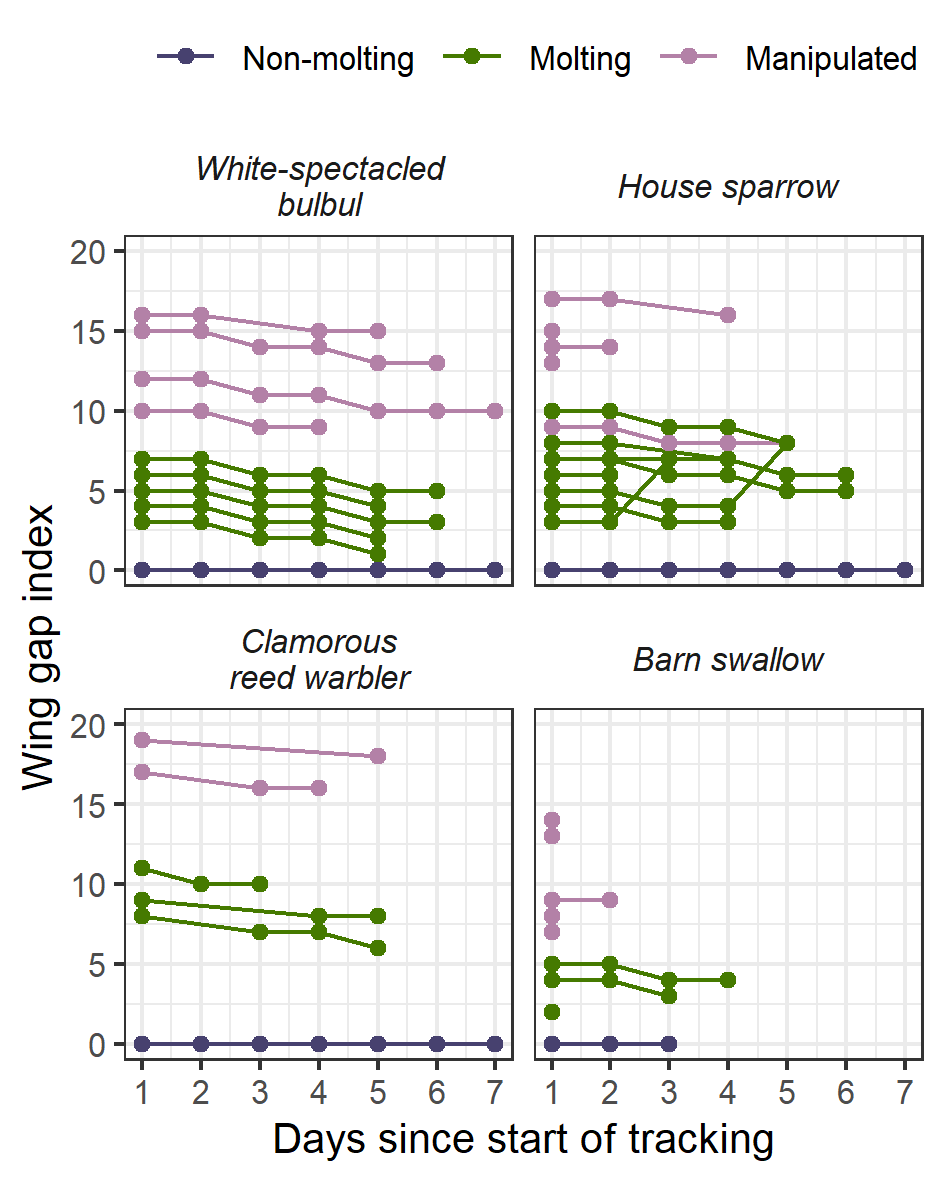
\includegraphics[width=0.5\textwidth]{figures/holeybirds/fig_spm_01}
    \caption{
        \textbf{Forecast daily change in wing gap index, per individual.}
        The size of the molt-related wing gap decreases slowly and constantly as feathers regrow, but the wing gap size may also increase in gradual jumps as a feather is shed during molt.
        We calculated the mean daily progress in the molt score, based on a sample of individuals of each species documented twice during the molt process.
        For each bird included in the study, we calculated the expected daily change in molt-related wing gap size based on the measurement we made at the time of tagging (day 1 in each panel).
    }
    \label{fig:wgi-daily}
\end{figure}

\section*{Vegetation, visibility, and land use across the study area}

\subsection*{Land cover}

We manually constructed spatial polygons of the land-cover types in our study area, based on aerial imagery and field experience (see Fig.~\ref{fig:hula-maps}A).
We categorised the study area into five main land-cover classes: settlements and built-up areas, open or agricultural areas, naturally occurring reedbeds, areas with trees (including orchards), and water (including canals and streams). 

\subsection*{Vegetation Productivity}

We obtained a standard measure of vegetation productivity, the normalised difference vegetation index (NDVI), which is widely used in animal ecology \parencite{pettorelli2011}.
We did this by accessing the European Space Agency Copernicus mission's Sentinel 2 imagery from the multi-spectral instrument, at a resolution of 10m.
We accessed data from the Level-1C collection, which covered the study area during the period in which we were interested (June -- October, 2016), rather than using the somewhat better Level-2A data, which covers the study area only from 2017 onwards.
We calculated NDVI using the standard formula $\text{NDVI} = (\text{NIR} - \text{Red}) / (\text{NIR} + \text{Red})$, where \textit{NIR} is the near infra-red band, and \textit{Red} is the red band.
We used Sentinel band 8 (near infra-red; 835.1 nm or 833 nm) and band 4 (red; 664.5 nm or 665 nm) to
calculate NDVI, with minor differences in the band wavelengths due to small differences between the two Sentinel-2 satellites, S2A and S2B.
We performed the full pipeline of NDVI calculation on Google Earth Engine \parencite{gorelick2017}, using the Python API (http://code.google.com/p/earthengine-api/) and the \textit{geemap} library \parencite{wu2020}.
NDVI across our study area varied between small negative values (indicating water), 0 (usually indicating bare ground), and large positive values up to 0.7 (indicating strong vegetation growth; see Fig.~\ref{fig:hula-maps}B).
The largest NDVI values were associated with some agricultural fields, as well as with orchards with growing trees, and with natural reedbeds (compare see Fig.~\ref{fig:hula-maps}A -- B; see correlation below).

\subsection*{Visibility Index}

We obtained a canopy height model (CHM) of the majority of our study area from the Survey of Israel at 50cm resolution.
We could not access CHM data for some peripheral areas as this is a border region.
In contrast to the more conventional elevational model, CHMs can pick up fine-scale variation in the heights of objects above the ground surface.
This makes CHMs suitable for investigating animals' interactions with their three-dimensional environment, with substantial spatial detail.
CHMs are especially useful in exploring how animal movement decisions are linked to animals' lines of sight \parencite{aben2018,aben2021}.
We used the Visibility Index plugin v1.2 (https://github.com/zoran-cuckovic/QGIS-visibility-analysis) for QGIS v3.x (i.e., 3.0 or higher) to calculate the visibility index across the CHM.
We downsampled the CHM to 1m resolution to speed up computation without losing much detail.
We used an observer height of 1.5 m above the canopy surface; this is the height above either the actual tree canopy, or over any other surface present in our landscape (water, open fields, settlements etc.).
We used an observer perception distance of 50 m, and calculated the proportion of 16 surrounding angles from which any cell of the CHM could be observed (option \textit{Incoming Views}).
This yielded a layer with as many cells as the CHM, and with the same (1 m) resolution, with values of the visibility between 0 and 1.

In biological terms, the visibility index is an estimate of how exposed any location is to a low-flying aerial predator, up to 50 m away.
We modelled these values based on the hunting flights of a common bird-preying raptor, the Eurasian sparrowhawk \parencite[\textit{Accipiter nisus}][]{seress2011,krams2001,krams2020}.
We also considered the visibility index of our study site from the point of view of a typically high-flying raptor, the common kestrel (\textit{Falco tinnunculus}), and repeated the visibility index calculations for an observer height of 15m (Fig.~\ref{fig:hula-maps}D).
Kestrels hovering above the landscape surface are conspicuous to prey species whose avoidance mechanisms are primarily visual, such as small birds which rely on spotting predators early and taking cover \parencite{krams2001,krams2020}.
Thus the strategy of bird-preying raptors such as sparrowhawks is to fly low over the landscape surface (canopy or ground), and to attempt to surprise birds while they have broken cover \parencite{krams2001,seress2011,krams2020}.
Accounting for these natural history and behavioural aspects of birds' predator-prey interactions, we chose the 1.5m visibility index layer for our analyses.

The visibility index of locations in our study area was strongly tied to land-cover, as expected (Fig.~\ref{fig:hula-maps}C; compare Fig.~\ref{fig:hula-maps}A).
Agricultural areas have visibility index values $\approx$1.0, and are unlikely to offer much shelter from aerial predators.
Orchards and areas of natural vegetation such as reedbeds are much more sheltered, with visibility index values $<$ 0.2.
Built-up areas such as settlements, surprisingly, have lower visibility scores than open agricultural fields, as human-made structures are relatively tall and effectively obstruct the lines of sight of predators (Fig.~\ref{fig:hula-maps}C; compare Fig.~\ref{fig:hula-maps}A).

\begin{figure}
    \centering
    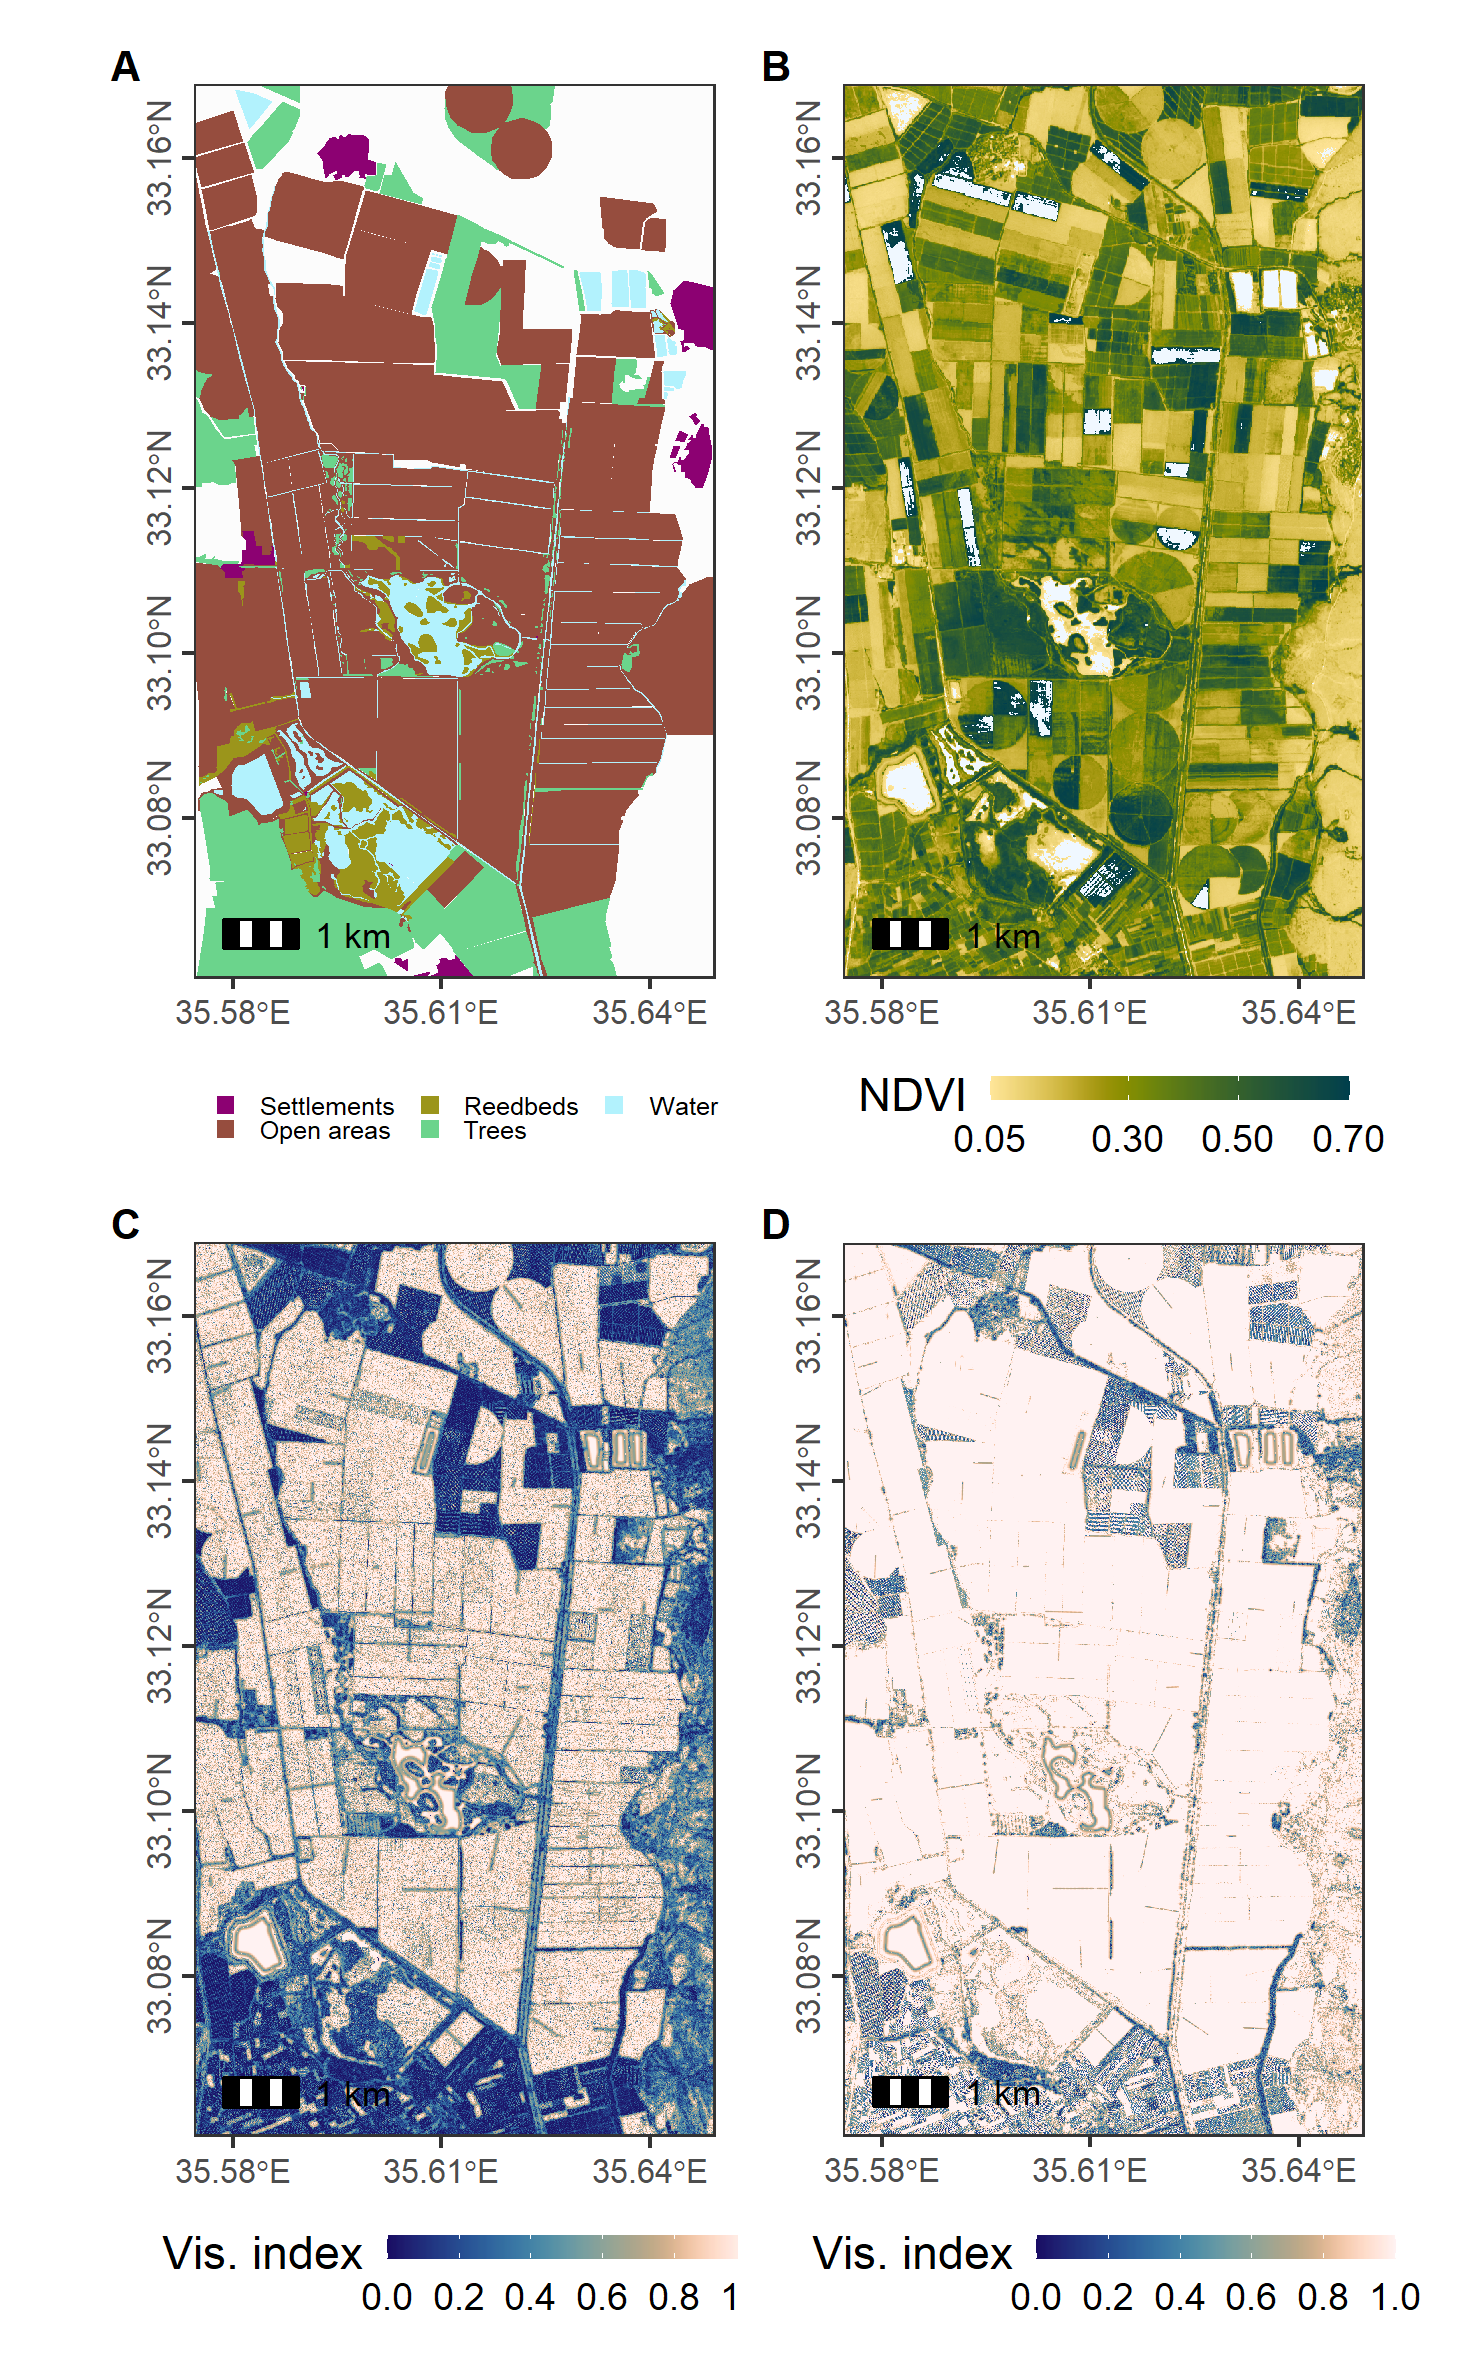
\includegraphics[width=0.7\textwidth]{figures/holeybirds/fig_spm_02}
    \caption{
        \textbf{Vegetation productivity, exposure to potential predators, and land-cover across the Hula Valley, Israel.}
        \textbf{(A)} Our study site in the Hula Valley in northern Israel is an agricultural-natural habitat matrix.
        \textbf{(B)} There is substantial fine-scale variation in vegetation cover and productivity (here, the normalised difference vegetation index: NDVI), even within areas of similar land-cover. Areas shown in white are water bodies.
        \textbf{(C)} Despite substantial areas being covered by growing vegetation, the majority of the study area is relatively exposed to a low-flying aerial predator (such as Eurasian sparrowhawk \textit{Accipiter nisus}, with a visibility index score $\approx$1.0. Sheltered areas, with lower visibility index scores ($<$ 0.4), form fine-scale refugia within the agricultural landscape.
        However, areas covered by fruit tree orchards are very sheltered from low-flying predators, with visibility index scores $<$ 0.2.
        \textbf{(D)} The visibility of an area is strongly dependent on the height of the observer, and nearly the entire study area is heavily exposed to a high-flying aerial predator such as the common kestrel (\textit{Falco tinnunculus}), hovering at 15m above the surface.
        However, this also makes high-flying predators conspicuous to visually oriented prey such as small birds.
        To counter this, bird-preying raptors such as sparrowhawks typically fly at low heights to surprise small birds emerging from cover.
    }
    \label{fig:hula-maps}
\end{figure}

\subsection*{Relationship between Vegetation Productivity and Visibility}

Fine-scale variation in vegetation structure, and especially in plant height, creates three-dimensional habitat complexity, which translates into the sheltering effect of vegetated habitats.
This suggests that vegetation indices such as NDVI could be used to examine the availability of shelter.
We tested this hypothesis by examining the relationship between NDVI and the visibility index using a generalised additive model (GAM).
We extracted the NDVI, visibility index, and land-cover type for 10,000 equally spaced locations across our study area, and excluded areas which were covered by water.
We fit a GAM with the formula: 
\begin{linenomath*}
    $$\text{visibility~index} \sim s(\text{NDVI}, by = \text{landcover}) + s(\text{landcover}, bs = \text{``re''})$$
\end{linenomath*}
This fit a separate smooth visibility-NDVI curve for each land-cover class, and also modelled land-cover as a random effect \parencite{wood2017}.

We found that the relation between NDVI and visibility index was statistically significant, but the shape of the relationship was strongly influenced by land-cover (Fig.~\ref{fig:vis-ndvi}; GAM degrees of freedom [DOF] = 2.99, estimate $F$ = 1,004.02, p $<$ 0.001; $R^2$ = 0.596).
In areas covered by trees, NDVI values $>$ 0.2 were uniformly associated with low visibility ($<$ 0.25), and thus, potentially more shelter from aerial predators (GAM DOF = 5.117, estimate $F$ = 28.0, p $<$ 0.001).
In natural reedbeds, we found a nearly linear relationship, with visibility declining with increasing NDVI (GAM DOF = 2.227, estimate $F$ = 27.13, p $<$ 0.001).
Surprisingly, in settlements and built-up areas, visibility was consistently $<$ 0.5, despite relatively low NDVI values overall $<$ 0.5 (GAM DOF = 1.0, estimate $F$ = 14.85, p $<$ 0.001).
This is likely because tall structures such as houses block lines of sight quite effectively.
Agricultural fields and open areas had predictably high visibility values ($>$ 0.7) regardless of their NDVI values (GAM DOF = 6.827, estimate $F$ = 26.41, p $<$ 0.001).
Overall, in landscapes with mixed vegetation types, or with substantial topological complexity, NDVI does not have a simple relationship with the availability of shelter (GAM DOFs $>$ 1.0).
Selection for NDVI in animal movement studies should thus be interpreted as selection for shelter only with some caution.
It is more accurate to obtain and use canopy height models to calculate visibility indices and so to get an estimate of shelter with a basis in the mechanisms of visual cognition.
Where this is challenging, such as at larger spatial scales, accounting for land-cover in habitat selection models may be one alternative.

\begin{figure}
    \centering
    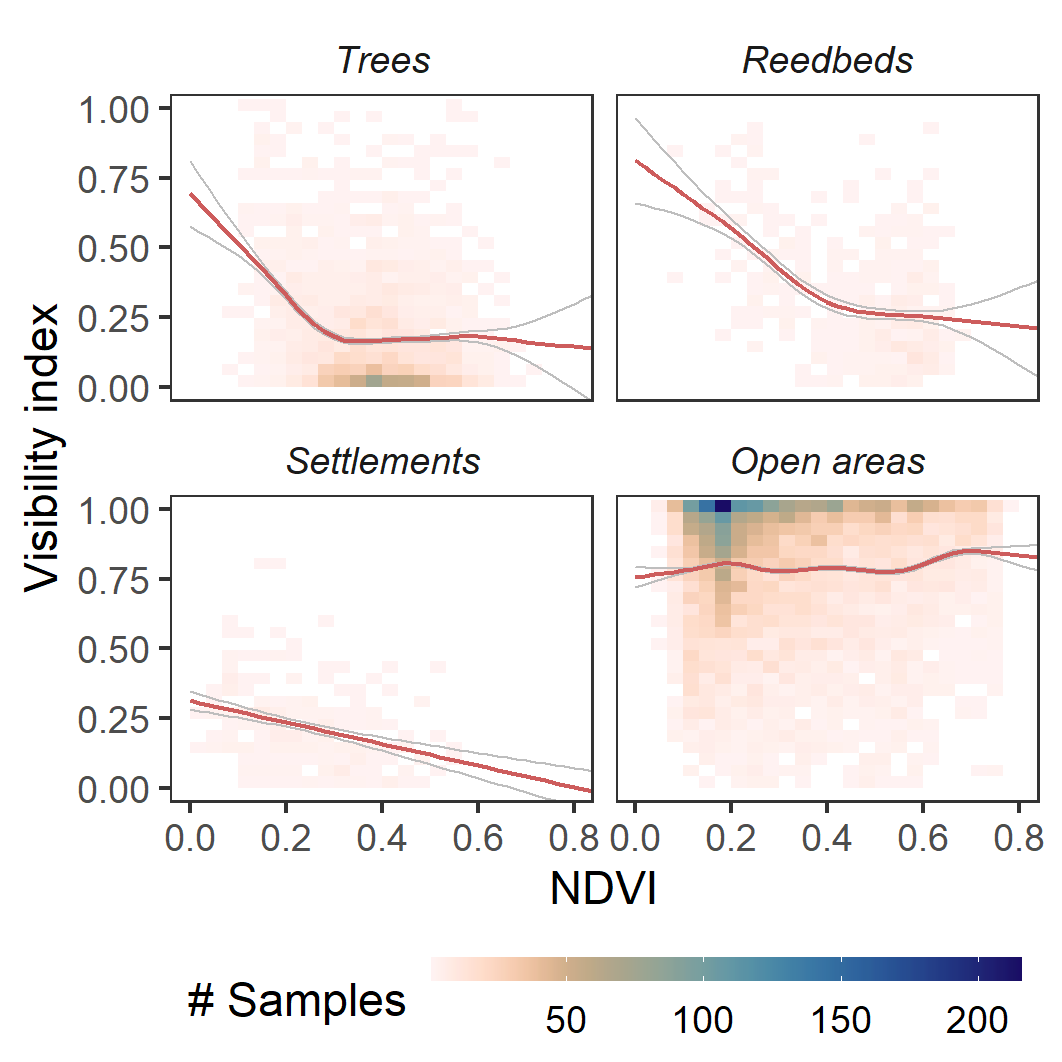
\includegraphics[width=0.5\textwidth]{figures/holeybirds/fig_spm_03}
    \caption{Generalised additive model fits showing the relationship between NDVI and the visibility index. Visibility index shown here was calculated with an observer height of 1.5m, which is representative of the hunting flight of bird-preying raptors (see Fig. S2C).}
    \label{fig:vis-ndvi}
\end{figure}

\section*{Modelling the Effect of Wing Gap Size on Large-scale Movements}

We modelled the effect of wing gap size, given by the wing gap index, on large-scale movements using GAMs.
We examined data from four non-migratory birds common to our study area in northern Israel: barn swallows (\textit{Hirundo rustica}), white-spectacled bulbuls (\textit{Pycnonotus xanthopygos}), house sparrows (\textit{Passer domesticus}), and clamorous reed warblers (\textit{Acrocephalus stentoreus}).
For bulbuls, sparrows, and reed warblers, we fit one GAM with species-specific curves to relate the average hourly distance moved between areas of prolonged residence \parencite[``residence patches''][]{gupte2022d}, and the individual wing gap index
We used the GAM formula:
\begin{linenomath*}
    $$
        \text{distance between patches per hour} \sim s(\text{wing gap index}, by = \text{species}, k = 3) +\\
    s(\text{species}, bs = \text{``re''})      
    $$
\end{linenomath*}
This fit a GAM with wing gap index as a smoothed term with three knots allowed, and species as a random effect \parencite{wood2017}.
Model coefficients are in Table~\ref{table:coef_distance}.

\begin{table}
    \begin{center}
    \begin{tabular}{l D{)}{)}{11)3}}
    \hline
     & \multicolumn{1}{c}{Coefficients} \\
    \hline
    Intercept          & 136.89 \; (60.97)^{*} \\
    WGI - bulbul       & 1.90 \;  (1.99)^{*}   \\
    WGI - sparrow      & 1.92 \;  (1.99)^{***} \\
    WGI - warbler      & 1.00 \;  (1.00)       \\
    Species            & 1.96 \;  (2.00)^{***} \\
    \hline
    AIC                & 2590.40               \\
    BIC                & 2619.82               \\
    Log Likelihood     & -1286.41              \\
    Deviance           & 2573521.55            \\
    Deviance explained & 0.52                  \\
    Dispersion         & 12726.89              \\
    R$^2$              & 0.50                  \\
    GCV score          & 13217.10              \\
    Num. obs.          & 210                   \\
    Num. smooth terms  & 4                     \\
    \hline
    \multicolumn{2}{l}{\scriptsize{$^{***}p<0.001$; $^{**}p<0.01$; $^{*}p<0.05$}}
    \end{tabular}
    \caption{Generalised additive model coefficients for distance between residence patches.}
    \label{table:coef_distance}
    \end{center}
\end{table}

To determine whether the molt-related wing gap's size also affected the frequency with which birds moved from one putative foraging patch to another, we fit a GAM to the number of patch switches (essentially, the number of patches) per hour of daytime tracking, using the formula:
\begin{linenomath*}
    $$
        \text{number of patches visited per hour} \sim s(\text{wing gap index}, by = \text{species}, k = 3) +\\
    s(\text{species}, bs = \text{``re''})
    $$
\end{linenomath*}
Model coefficients are in Table~\ref{table:coef_switches}.
For swallows, we fit a GAM with distance travelled per hour of tracking as the response, and the individual wing gap index as the smooth predictor.
This fit a GAM with wing gap index as a smoothed term with three knots allowed:
\begin{linenomath*}
$$\text{distance per hour} \sim s(\text{wing gap index}, k = 3)$$
\end{linenomath*}
These results are reported in the main text.

\begin{table}
    \begin{center}
    \begin{tabular}{l D{)}{)}{8)3}}
    \hline
     & \multicolumn{1}{c}{Coefficients} \\
    \hline
    Intercept          & 0.76 \; (0.13)^{***} \\
    WGI - bulbul       & 1.93 \; (2.00)^{**}  \\
    WGI - sparrow      & 1.36 \; (1.59)^{*}   \\
    WGI - warbler      & 1.00 \; (1.00)       \\
    Species            & 1.92 \; (2.00)^{***} \\
    \hline
    AIC                & 175.48               \\
    BIC                & 202.97               \\
    Log Likelihood     & -79.52               \\
    Deviance           & 26.22                \\
    Deviance explained & 0.29                 \\
    Dispersion         & 0.13                 \\
    R$^2$              & 0.27                 \\
    GCV score          & 0.13                 \\
    Num. obs.          & 210                  \\
    Num. smooth terms  & 4                    \\
    \hline
    \multicolumn{2}{l}{\scriptsize{$^{***}p<0.001$; $^{**}p<0.01$; $^{*}p<0.05$}}
    \end{tabular}
    \caption{Generalised additive model coefficients for residence patch switches.}
    \label{table:coef_switches}
    \end{center}
\end{table}

\section*{Modelling the Effect of Wing Gap Size on Patch Occupancy}

We examined whether birds' molt-related wing gap size affected the duration that they spent in each residence patch.
Following from the results of the models described above (see main text Figs. 1 -- 2), we expected that molting birds would spend a shorter duration in each patch, as this is the only way to achieve both farther distances between patches, as well as more frequent patches, given a constant flight speed.
We fit a GAM to the duration (in hours) of each residence patch as:
\begin{linenomath*}
    $$
        \text{patch duration} \sim s(\text{wing gap index}, by = \text{species}, k = 3) + \\
        \text{visibility index} + \text{ndvi} +
        s(\text{species}, bs = \text{``re''})
    $$
\end{linenomath*}
Here, we also included the visibility index and NDVI as parametric fixed effects.
Model coefficients are in Table~\ref{table:coef_duration}.

\begin{table}
    \begin{center}
    \begin{tabular}{l D{)}{)}{9)3}}
    \hline
     & \multicolumn{1}{c}{Coefficients} \\
    \hline
    Intercept          & 1.15 \; (0.20)^{***}  \\
    Visibility index   & -0.80 \; (0.21)^{***} \\
    NDVI               & 0.09 \; (0.27)        \\
    WGI - bulbul       & 1.98 \; (2.00)^{***}  \\
    WGI - sparrow      & 1.00 \; (1.00)        \\
    WGI - warbler      & 1.82 \; (1.96)^{*}    \\
    Species            & 1.84 \; (2.00)^{***}  \\
    \hline
    AIC                & 6919.17               \\
    BIC                & 6979.39               \\
    Log Likelihood     & -3448.94              \\
    Deviance           & 3230.34               \\
    Deviance explained & 0.06                  \\
    Dispersion         & 1.53                  \\
    R$^2$              & 0.06                  \\
    GCV score          & 1.54                  \\
    Num. obs.          & 2115                  \\
    Num. smooth terms  & 4                     \\
    \hline
    \multicolumn{2}{l}{\scriptsize{$^{***}p<0.001$; $^{**}p<0.01$; $^{*}p<0.05$}}
    \end{tabular}
    \caption{Generalised additive model coefficients for residence patch duration.}
    \label{table:coef_duration}
    \end{center}
\end{table}

\section*{Modelling the Effect of Wing Gap Size on Visibility of Residence Patches}

We fit GAMs with species-specific smooths to examine the effect of wing gap size on the availability of shelter in individual birds' residence patches.
We included NDVI as a smoothed term to account for the effect of vegetation productivity, using the formula:
\begin{linenomath*}
$$ \text{visibility} \sim s(\text{wing gap index}, by = \text{species}, k = 3) + \\
    s(\text{NDVI}, k = 5) + s(\text{species}, bs = \text{``re''})
$$
\end{linenomath*}
Here, the wing gap index is allowed 3 knots, while NDVI is allowed five knots for a potentially more complex relationship.
We did not find a significant effect of wing gap index on species' use of more sheltered patches.
The one exception was clamorous reed warblers, in which the visibility of residence patches decreased linearly with increasing wing gap index (GAM DOF = 1.0 [a linear fit], $F$ = 16.354, p < 0.001).
Full model coefficients are reported in Table~\ref{table:coef_vis}.
NDVI had a significant, non-linear relationship with visibility, as expected from our analysis of the visibility-NDVI relationship above (GAM DOF = 3.885, $F$ = 172.493, p < 0.001).
Model results are version controlled at \textit{github.com/pratikunterwegs/holeybirds} in the file ``data/results/mod\_summary\_rrv\_visibility.txt''

\begin{table}
    \begin{center}
    \begin{tabular}{l D{)}{)}{8)3}}
    \hline
     & \multicolumn{1}{c}{Coefficients} \\
    \hline
    Intercept          & 0.33 \; (0.02)^{***} \\
    NDVI               & 1.00 \; (1.00)^{**}  \\
    WGI - bulbul       & 1.00 \; (1.00)       \\
    WGI - sparrow      & 1.76 \; (1.94)       \\
    WGI - warbler      & 3.90 \; (3.99)^{***} \\
    Species            & 1.88 \; (2.00)^{***} \\
    \hline
    AIC                & -2108.51             \\
    BIC                & -2046.84             \\
    Log Likelihood     & 1065.79              \\
    Deviance           & 22.94                \\
    Deviance explained & 0.35                 \\
    Dispersion         & 0.01                 \\
    R$^2$              & 0.34                 \\
    GCV score          & 0.02                 \\
    Num. obs.          & 1550                 \\
    Num. smooth terms  & 5                    \\
    \hline
    \multicolumn{2}{l}{\scriptsize{$^{***}p<0.001$; $^{**}p<0.01$; $^{*}p<0.05$}}
    \end{tabular}
    \caption{Generalised additive model coefficients for residence patch visibility.}
    \label{table:coef_vis}
    \end{center}
\end{table}

\section*{Examining the Effects of Visibility and Vegetation Productivity on Habitat Selection}

Finding a correlation between vegetation growth in the form of NDVI, and visibility, we adopted a step-selection approach \parencite{fieberg2010,signer2019,fieberg2021} to disentangle the effects of these two factors on the movements of molting birds.
We performed this analysis on the movements of bulbuls, sparrows, and reed warblers between their residence patches.
We excluded swallows because we had not constructed residence patches for these birds, and because we could not resolve their flight altitude, making it difficult to determine whether they were using shelter.

We drew 9 alternative patch movements for every real patch movement, that is from patch $N$ to patch $N+1$, and sampled 15 locations distributed around the alternative moves.
We drew the locations of the 9 alternative movements by drawing first a distance from a gamma distribution fitted to each individual's daily movements between patches, and second, an angle drawn from a von Mises distribution fitted to the individual's turning angles during large-scale movements between patches (see main text Fig. 1).
For each of these alternative moves, we drew 15 locations from a normal distribution centred on the coordinates of the move, with a standard deviation of 20 m.
In this way, we constructed `alternative residence patches', which we could compare with the patches that birds actually used.
At each of the 135 alternative locations (15 locations $\times$ 9 patches) we obtained the NDVI and visibility index.

We compared the NDVI and visibility of the 15 points in each potential patch, with the NDVI and visibility of a flexible number of real positions of patches actually used by individuals, by fitting a conditional logistic regression to the patch status (real or alternative).
On average, across species and molt status, there were 28.1 real positions (SD = 25.3) compared against 251 potential positions (SD = 228).
In this way, we were able to determine how birds selected for vegetation productivity and shelter when moving.
Since most birds' residence patches are in high-NDVI low-visibility areas (see main text Fig. 4), but are surrounded by high-NDVI, high-visibility areas, this allowed us to disentangle the provisioning effects of vegetation from its sheltering effects.

We fit separate regressions for each molt status for each of the three species, using the formula:
\begin{linenomath*}
$$ \text{case\_} \sim \text{visibility} + \text{NDVI} + \text{strata}(\text{step~identity}) $$
\end{linenomath*}
We chose the ``approximate'' fitting method to reduce computational time.
Model coefficients are presented in Table~\ref{table:coef_ssa}; negative coefficients indicate selection against visibility, and for shelter.

\begin{sidewaystable}
    \setlength{\tabcolsep}{4pt}
    
    \begin{center}
    
        \resizebox{\textwidth}{!}{%
        \begin{tabular}{l D{.}{.}{3.5} D{.}{.}{4.5} D{.}{.}{4.5} D{.}{.}{4.5} D{.}{.}{4.5} D{.}{.}{4.5} D{.}{.}{3.3} D{.}{.}{4.5} D{.}{.}{3.4}}
        \toprule
        & \multicolumn{3}{c}{White-spectacled bulbul} & \multicolumn{3}{c}{House sparrow} & \multicolumn{3}{c}{Clamorous reed warbler} \\
        \cmidrule(lr){2-4} \cmidrule(lr){5-7} \cmidrule(lr){8-10}
        & \multicolumn{1}{c}{Non-moulting} & \multicolumn{1}{c}{Molting} & \multicolumn{1}{c}{Manipulated} & \multicolumn{1}{c}{Non-moulting} & \multicolumn{1}{c}{Molting} & \multicolumn{1}{c}{Manipulated} & \multicolumn{1}{c}{Non-moulting} & \multicolumn{1}{c}{Molting} & \multicolumn{1}{c}{Manipulated} \\
        \midrule
        Visibility index & -8.27^{***} & -5.01^{***} & -5.84^{***} & -5.34^{***} & -6.68^{***} & -3.90^{***} & -3.58^{*} & -5.46^{***} & -16.78^{**} \\
                        & (1.70)      & (0.51)      & (0.56)      & (0.29)      & (0.67)      & (0.41)      & (1.44)    & (0.81)      & (5.39)      \\
        NDVI             & -0.45       & 0.99        & -1.47       & -0.69^{*}   & 0.42        & -0.04       & 1.22      & -0.00       & -3.04       \\
                        & (1.57)      & (0.67)      & (0.84)      & (0.35)      & (0.82)      & (0.70)      & (2.33)    & (1.20)      & (6.77)      \\
        \midrule
        AIC              & 279.66      & 3014.80     & 1874.35     & 5333.12     & 1190.49     & 1173.51     & 421.54    & 977.53      & 90.57       \\
        R$^2$            & 0.12        & 0.08        & 0.09        & 0.10        & 0.12        & 0.08        & 0.06      & 0.09        & 0.13        \\
        Max. R$^2$       & 0.55        & 0.67        & 0.63        & 0.68        & 0.58        & 0.61        & 0.57      & 0.65        & 0.50        \\
        Num. events      & 42          & 300         & 209         & 522         & 164         & 140         & 54        & 103         & 16          \\
        Num. obs.        & 415         & 2983        & 2085        & 5209        & 1614        & 1373        & 538       & 1022        & 160         \\
        Missings         & 0           & 0           & 0           & 209         & 1           & 42          & 0         & 0           & 0           \\
        \bottomrule
        \multicolumn{10}{l}{\scriptsize{$^{***}p<0.001$; $^{**}p<0.01$; $^{*}p<0.05$}}
        \end{tabular}
        }
        \caption{Log relative selection strengths (RSS; also denoted by $\beta$) for patch visibility and NDVI.}
        \label{table:coef_ssa}
    \end{center}

\end{sidewaystable}

\endgroup

{ \begin{center} \barfont{-.-} \end{center} }

% \section*{Acknowledgments}

% This study was supported by the Minerva Center for Movement Ecology, the Minerva Foundation, and ISF grant ISF-965/15 to R.N and S.T, and ISF grant 1919/19 to S.T. We also thank the Survey of Israel for their generous help. 
% P.R.G was supported by an Adaptive Life Programme grant made possible by the Groningen Institute for Evolutionary Life Sciences (GELIFES), and by the European Research Council (ERC Advanced Grant No. 789240 awarded to F. J. Weissing).
% R.N also acknowledges support from the Adelina and Massimo Della Pergola Chair of Life Sciences.

% \newrefcontext[sorting=nyt]
% \section*{Literature Cited}
% \printbibliography[title={Literature~Cited},heading=none]
% \end{refsection}